Testing is limited to Unit and Usability Tests. It was agreed at the beginning of the project to not do UI testing since this is not so straight forward with Jetpack Compose. 

The Unit test focus on the Controller and the Actions which can be triggered by the View. The test coverage shows no test in the view package but a coverage of 45 of 48 functions in the Workbench Controller Class, which is where most of the logic is.

\begin{figure}[H]
\centering
\begin{subfigure}{.5\textwidth}
  \centering
  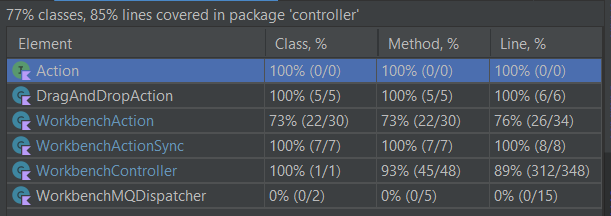
\includegraphics[width=.9\linewidth]{images/TestCoverageControllerPackage}
  \caption{Controller test Coverage}
  \label{fig:ransac_result}
\end{subfigure}%
\begin{subfigure}{.5\textwidth}
  \centering
  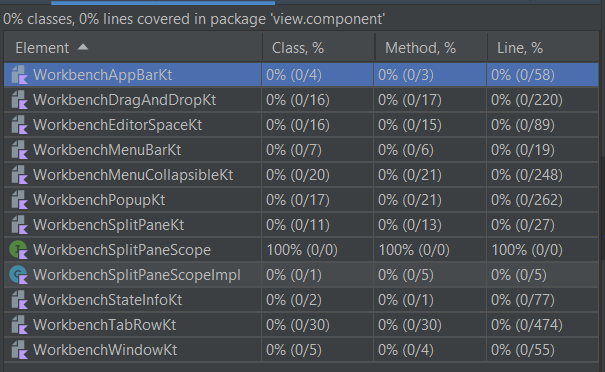
\includegraphics[width=.9\linewidth]{images/TestCoverageViewPackage.PNG}
  \caption{Explorer Space collapsed}
  \label{fig:ransac_rotation}
\end{subfigure}
\caption{View test Coverage}
\label{fig:ransac_results}
\end{figure}

\section{Usability Test}
The real estate example was created by Prof. Dr. Holz as part of a Usability test. This test led to changes around the Modules data handling and initialization.